\addcontentsline{toc}{section}{References}
\bibliographystyle{unsrt}
\bibliography{bibliography}

\addcontentsline{toc}{section}{\listfigurename}
\listoffigures

\addcontentsline{toc}{section}{\listtablename}
\listoftables

\printglossary[type=\acronymtype]
\printglossary

\appendix
\section{Appendix}
\label{part:appendix}

\begin{center}
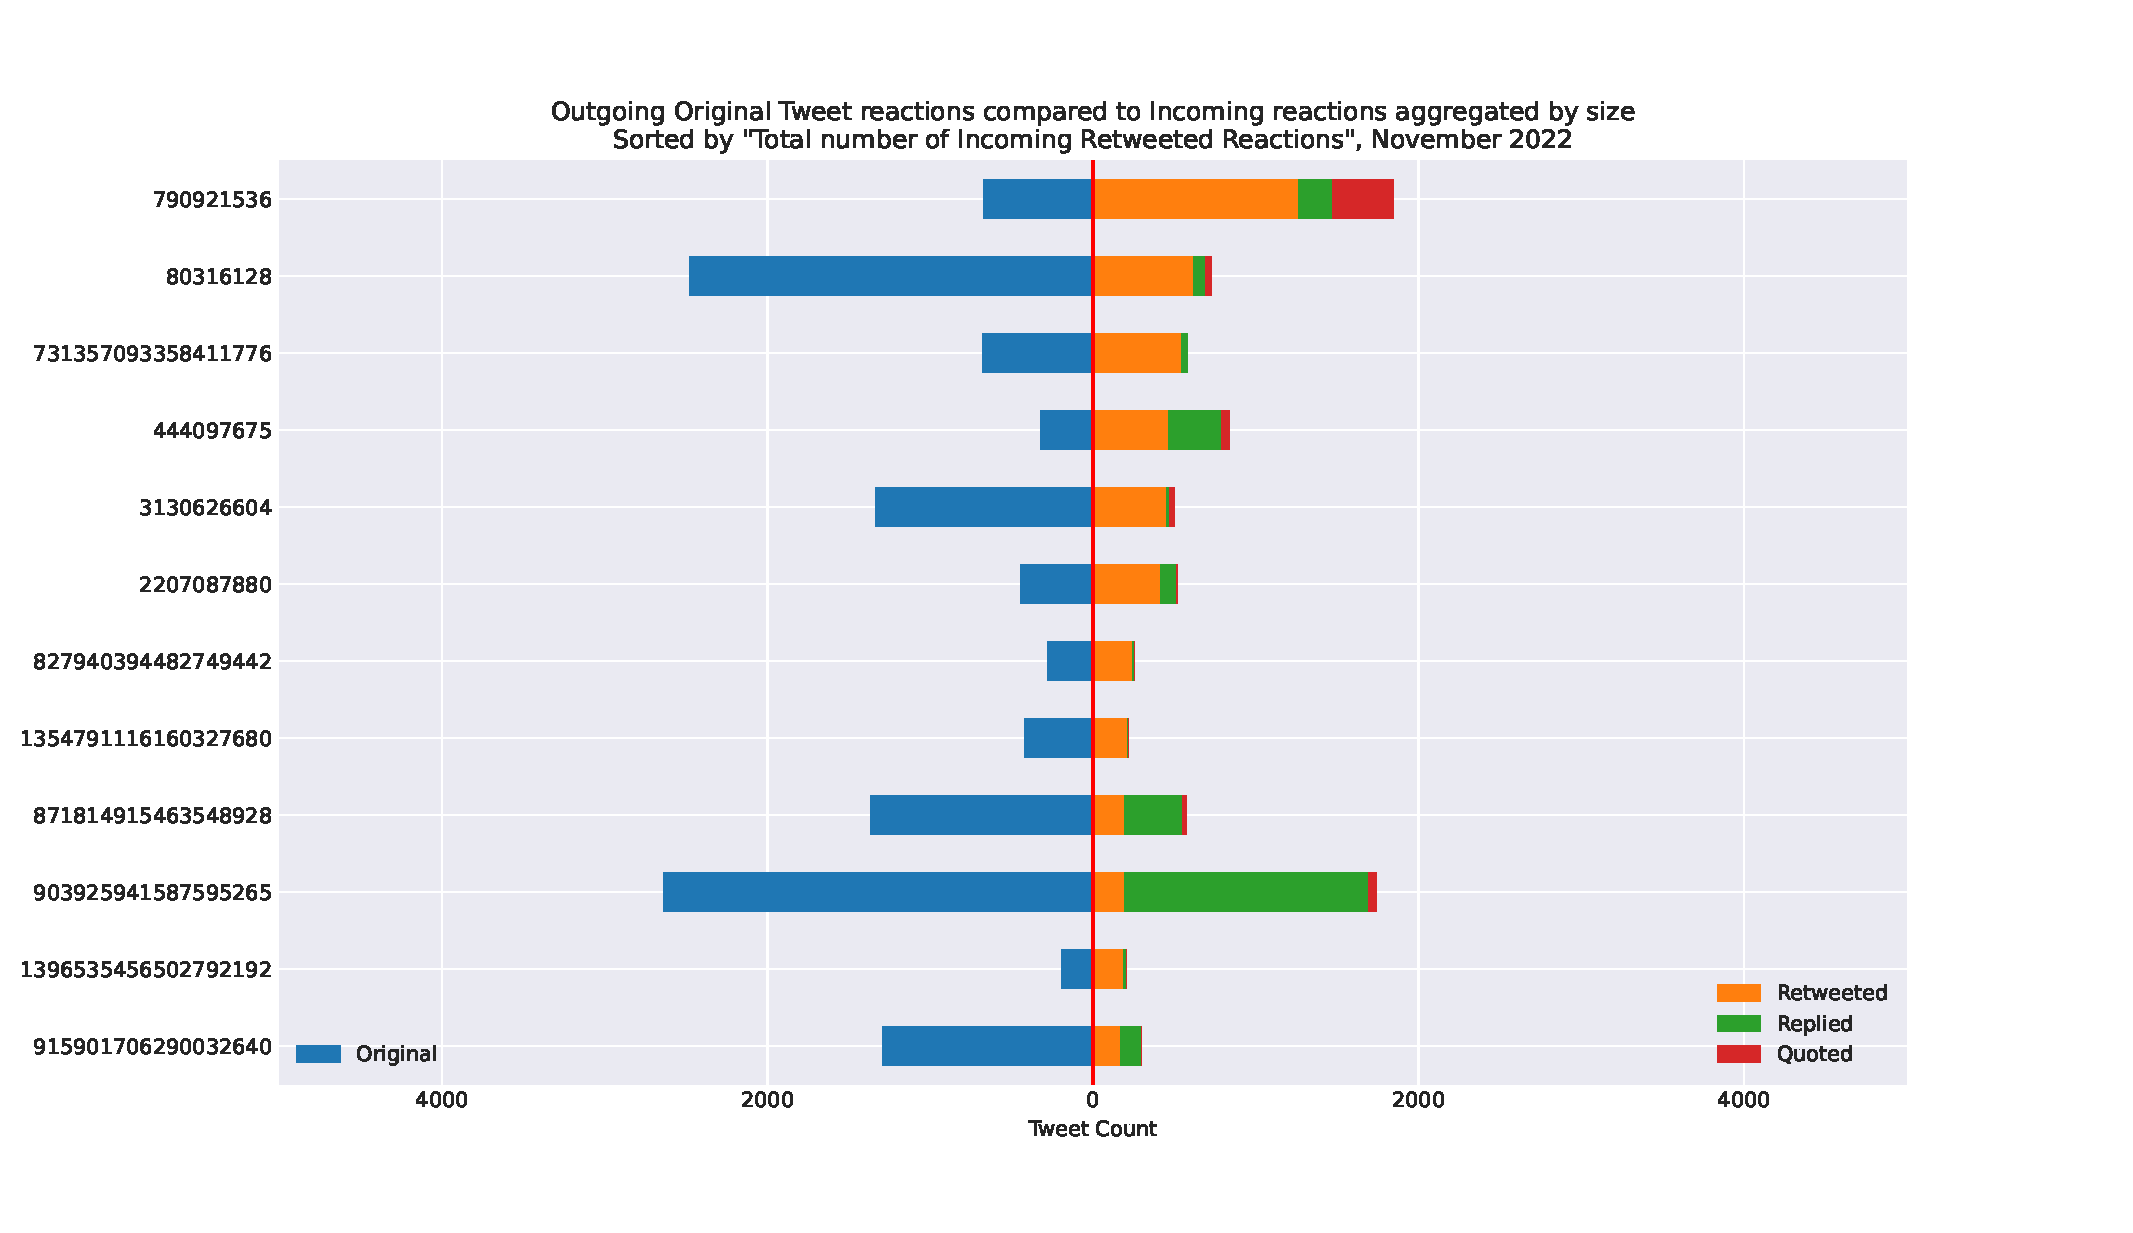
\includegraphics[width=16cm,keepaspectratio]{figures/users-retweet-in-initiators.eps}
\label{figure:users-retweet-in-initiators}
\captionof{figure}{Outgoing Original Tweet reactions compared to Incoming reactions aggregated by size. Referenced by: \ref{sec:results-tweets}}
\end{center}


\begin{center}
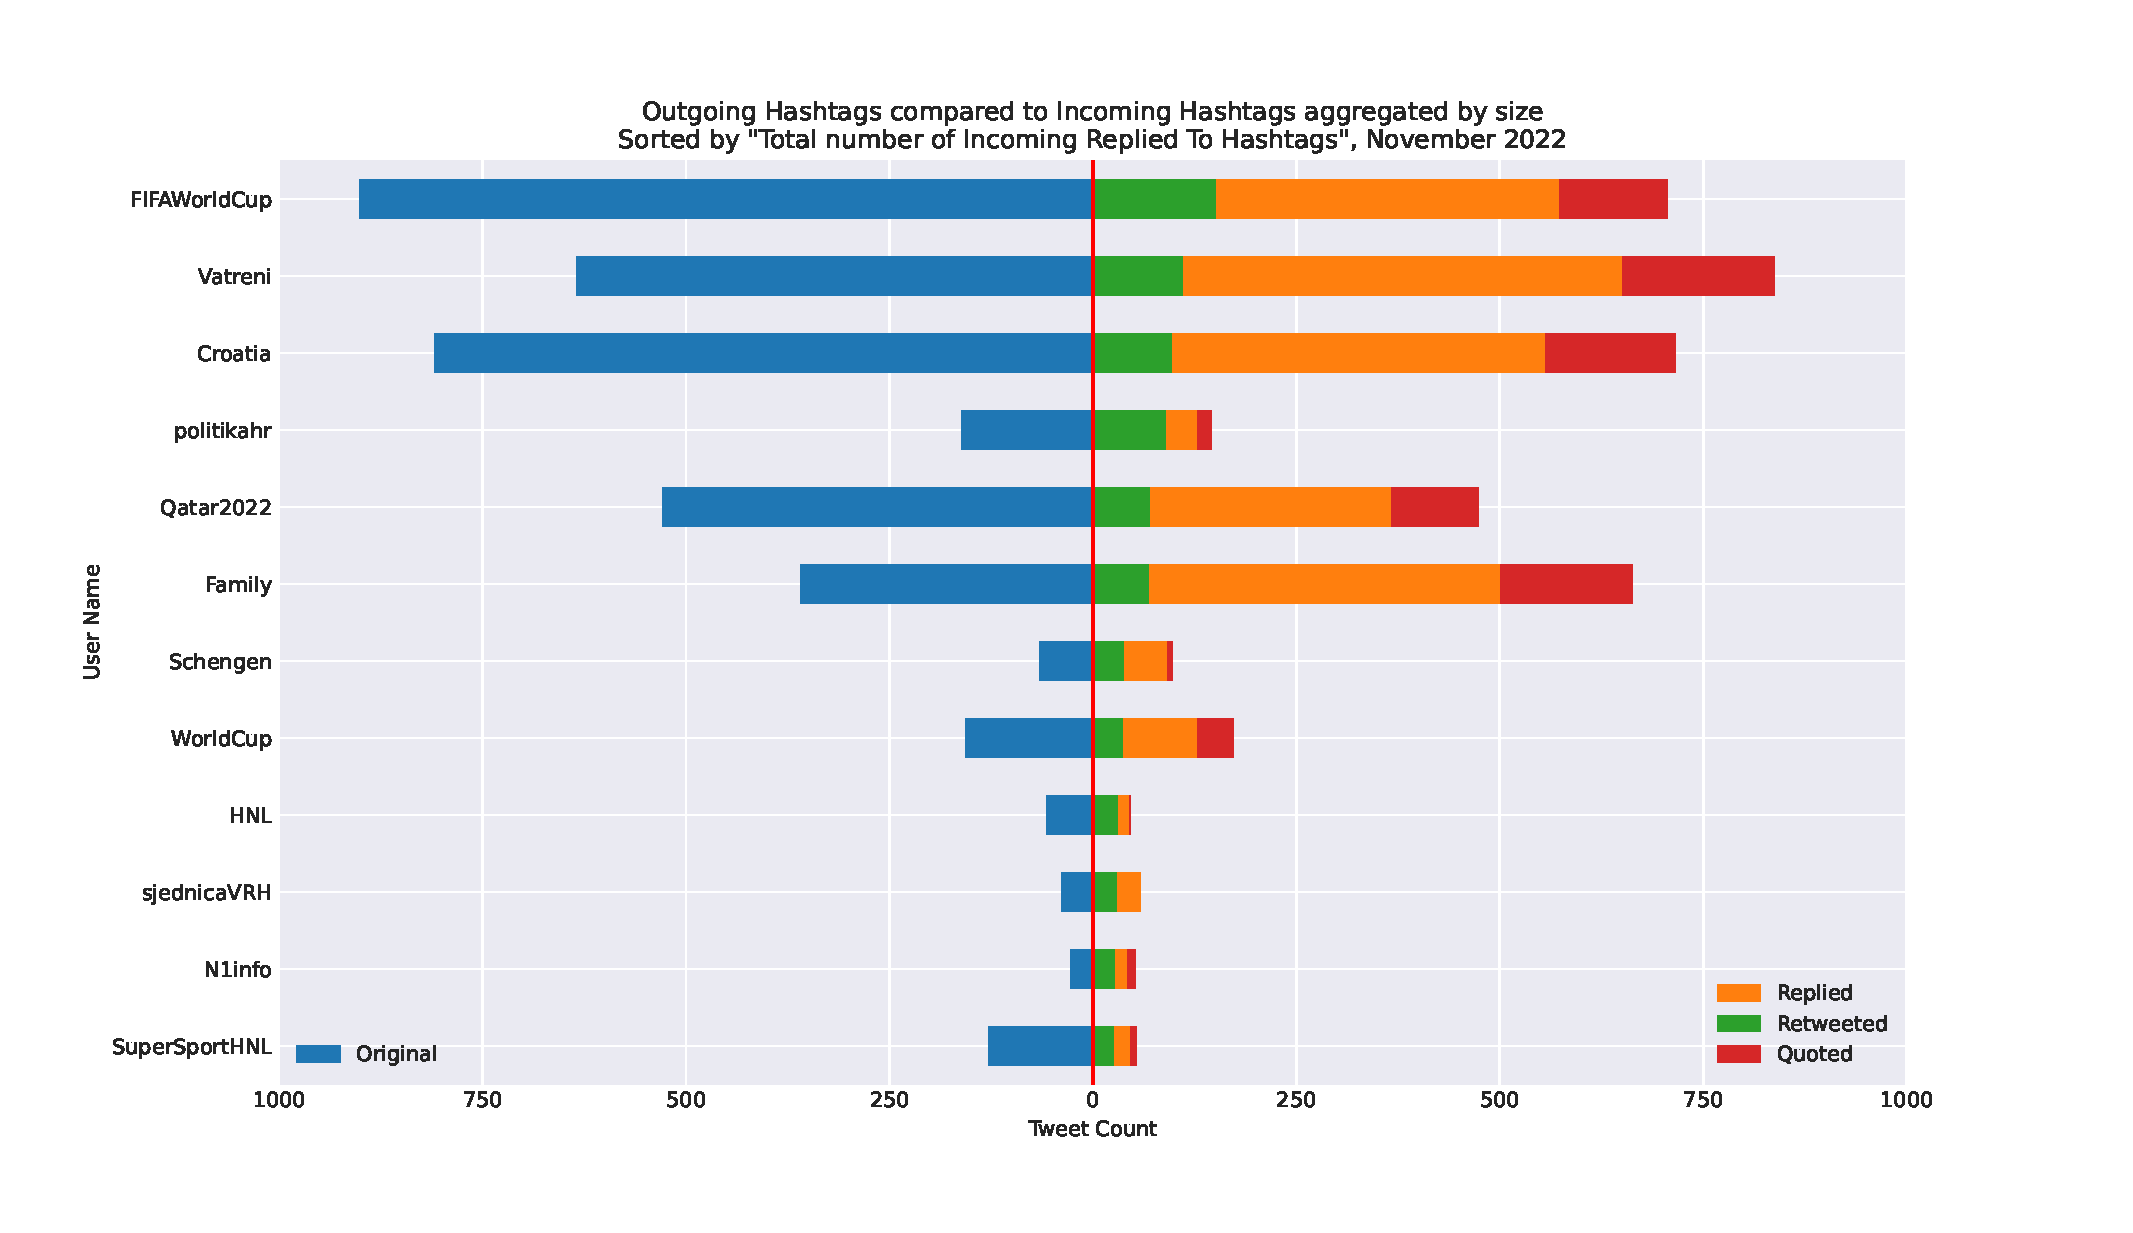
\includegraphics[width=16cm,keepaspectratio]{figures/hashtags-reply-in-reactions.eps}
\label{figure:hashtags-reply-in-reactions}
\captionof{figure}{Outgoing Hashtags compared to Incoming Hashtags aggregated by size. Referenced by: \ref{sec:results-hashtags}}
\end{center}

\begin{center}
\clearpage

\begin{table}[ht]
\caption{Correlations between measures describing selected subgraphs that represent "popular" or "not popular" content (1/2)}
\resizebox{\columnwidth}{!}{\begin{tabular}{l|r|r|r|r|r}
                                & avg\_degree       & avg\_in\_degree   & avg\_out\_degree  & avg\_betweenness\_centrality      & \textbf{popular}   \\ 
\hline
avg\_degree                     & 1.00              & -0.0127           & 0.8033            & 0.3901                            & 0.5936  \\ 
avg\_in\_degree                 & -0.0127           & 1.00              & -0.4716           & 0.0727                            & -0.7343 \\ 
avg\_out\_degree                & 0.8033            & -0.4716           & 1.00              & 0.1195                            & 0.8535  \\ 
avg\_betweenness\_centrality    & 0.3901            & 0.0727            & 0.1195            & 1.00                              & -0.1093 \\ 
avg\_clustering\_coeff          & -0.1040           & -0.8858           & 0.4877            & -0.3781                           & 0.6508  \\ 
betweenness\_centrality         & 0.4882            & -0.3122           & 0.4943            & 0.8708                            & 0.2703  \\ 
best\_pagerank                  & -0.2160           & 0.3393            & -0.4805           & 0.7365                            & -0.5966 \\ 
density                         & 0.2799            & 0.2963            & -0.0845           & 0.9650                            & -0.3435 \\ 
popular                         & 0.5936            & -0.7343           & 0.8535            & -0.1093                           & 1.00  \\ 
\hline
\end{tabular}}
\end{table}

\begin{table}[hb]
\caption{Correlations between measures describing selected subgraphs that represent "popular" or "not popular" content (2/2)}
\resizebox{\columnwidth}{!}{\begin{tabular}{l|r|r|r|r|r}
                                & avg\_clustering\_coeff    & betweenness\_centrality       & best\_pagerank    & density       & \textbf{popular}   \\
\hline
avg\_degree                     & -0.1040                   & 0.4882                        & -0.2160           & 0.2799        & 0.5936  \\
avg\_in\_degree                 & -0.8858                   & -0.3122                       & 0.3393            & 0.2963        & -0.7343 \\
avg\_out\_degree                & 0.4877                    & 0.4943                        & -0.4805           & -0.0845       & 0.8535  \\
avg\_betweenness\_centrality    & -0.3781                   & 0.8708                        & 0.7365            & 0.9650        & -0.1093 \\
avg\_clustering\_coeff          & 1.00                      & 0.0857                        & -0.5542           & -0.5694       & 0.6508  \\
betweenness\_centrality         & 0.0857                    & 1.00                          & 0.4665            & 0.7257        & 0.2703  \\
best\_pagerank                  & -0.5542                   & 0.4665                        & 1.00              & 0.8024        & -0.5966 \\
density                         & -0.5694                   & 0.7257                        & 0.8024            & 1.00          & -0.3435 \\
popular                         & 0.6508                    & 0.2703                        & -0.5966           & -0.3435       & 1.00  \\
\hline
\end{tabular}}
\end{table}
\label{table:graph-measures-correlation-matrix}
\end{center}
